\documentclass[11pt]{article}
\usepackage[margin=0.82in]{geometry}
\usepackage{amsmath,amssymb,amsthm,booktabs,longtable,graphicx,xcolor}
\usepackage[colorlinks=true,linkcolor=blue,urlcolor=blue]{hyperref}
\newtheorem{theorem}{Theorem}
\newtheorem{corollary}[theorem]{Corollary}
\newcommand{\F}{\mathbb F}
\newcommand{\OO}{\mathcal O}
\newcommand{\Nm}{N_-}
\newcommand{\Np}{N_+}
\title{Two genus-3 branches: exact class support and\newline verified representative construction}
\author{ISO-1 research evidence supplement}
\date{9 October 2026}
\begin{document}
\maketitle
\begin{abstract}
The linear and nonsplit quadratic branches of the published genus-3
hyperelliptic family admit complementary torus parametrizations of orders
$p^4+p^2+1$ and $p^4-p^2+1$. We prove their completeness, give an exact
CM intersection criterion for ordinary trace classes with fundamental
discriminant below $-4$, and implement both endpoint recognition and literal
model reconstruction. Complete censuses and independently sampled construction
receipts are reported separately. At $p=7$, the union contains 248 of 294
ordinary trace classes, including 122 classes absent from the cubic branch.
An independent native counter replays every retained parameter model by
48,118,441 affine-$x$ evaluations. The 192--252-bit experiment applies the
validated endpoint tests to all 512 previously frozen independent sources
in fields of degrees 6, 10 and 14.
\end{abstract}

\section{Contribution and relation to prior work}
Joux and Vitse use the genus-3 hyperelliptic family
\begin{equation}\label{family}
 y^2=h(x)(x-\alpha)(x-\alpha^q),\qquad
 \alpha\in K\setminus\F_q,\quad h\in\F_q[x],\quad \deg h\in\{1,2\},
\end{equation}
where $K=\F_{q^3}$ and $q=p^2$. Their cover and decomposition method supplies
the covering construction and destination algorithm \cite{JV}. Momose and
Chao already classify these coverings and study their density \cite{MC}.
The contribution here is an exact test for \emph{isogeny-class support} of
both branches, the resulting branch-aware census, and explicit source-to-family
routes with measured construction attempts on independent source models.
The earlier conductor restriction and census in this study concerned the
cubic norm-one branch. This supplement includes the nonsplit quadratic branch
in the same class decision.

Fields, coefficients and input laws are frozen in the companion raw receipts.
The construction experiment studies entire ordinary curve classes; a DLP
subgroup and generator are unspecified and remain null in its manifests.
Construction timings are shared-host resource diagnostics. The exact class
counts and algebraic checks do not depend on host isolation.

\section{Complete parametrization of both branches}
Write $Q=q^3$, $L=\F_{q^6}$ and
\[
 \Np=q^2+q+1,\quad \Nm=q^2-q+1,\quad
 j(\lambda)=\frac{256(\lambda^2-\lambda+1)^3}
 {\lambda^2(\lambda-1)^2}.
\]
Fix a nonsquare $d\in\F_q^\times$ and $\beta\in L$ with $\beta^2=d$.
Then $\beta^q=-\beta$ and $\beta^Q=-\beta$.

\begin{theorem}[Two-branch normalization and exact finite criterion]\label{normalize}
Let $p>3$ be prime. Up to $K$-isomorphism and quadratic twist, every
nonsingular model in \eqref{family} is either
\[
 E_\alpha:y^2=x(x-\alpha)(x-\alpha^q),
 \quad\text{or}\quad
 C_\alpha:y^2=(x^2-d)(x-\alpha)(x-\alpha^q).
\]
The cubic branch has the Legendre parameters
$\lambda\in\mu_{\Np}(K)\setminus\{1\}$. The quadratic branch has the
invariants $j(\lambda)$ for
$\lambda\in\mu_{\Nm}(L)\setminus\{1\}$.
For the quadratic branch set
\begin{equation}\label{reconstruct}
 a(q+1)\equiv1\pmod{\Nm},\qquad
 \gamma=\lambda^a,\qquad
 \alpha=\beta\frac{\gamma+1}{\gamma-1}.
\end{equation}
This constructs $\alpha\in K\setminus\F_q$ with invariant $j(\lambda)$.
Consequently, point-counting the two finite parameter sets and including both
quadratic twists gives an exact class-support criterion for \eqref{family}.
\end{theorem}

\begin{proof}
A degree-one $h$ is translated over $\F_q$ to a multiple of $x$.
A split squarefree quadratic is carried by an $\F_q$ M\"obius transformation
to a branch pair $0,\infty$, reducing to the same cubic case.
A nonsplit quadratic is translated and scaled over $\F_q$ to $x^2-d$:
the ratio of two nonsquares of $\F_q$ is a square. Each resulting nonzero
leading coefficient in $K$ has one of two square classes. Since $K/\F_q$
has odd degree, a base-field nonsquare remains a nonsquare in $K$.
Thus both leading-coefficient classes are represented by base-field twists.

For the cubic case, $\lambda=\alpha^q/\alpha$ has norm one.
Conversely Hilbert 90 constructs $\alpha$ from every nonidentity norm-one
$\lambda$; $\alpha\notin\F_q$ follows from $\lambda\ne1$.
Scaling $x$ by $\alpha$ gives its Legendre model up to twist.

For the quadratic case the Cayley map
\[
 \gamma=\frac{\alpha+\beta}{\alpha-\beta}
\]
is a bijection from $\mathbb P^1(K)$ to $\mu_{Q+1}(L)$.
It takes $\mathbb P^1(\F_q)$ to $\mu_{q+1}(L)$.
The map $\gamma\mapsto\gamma^{q+1}$ has kernel $\mu_{q+1}$ and image
$\mu_{\Nm}$, because $(q+1)\Nm=Q+1$.
Its nonidentity fibers therefore have exactly $q+1$ preimages, all outside
$\mathbb P^1(\F_q)$; there are $Q-q=(q+1)(\Nm-1)$ such preimages.
The cross-ratio of the four roots $\beta,-\beta,\alpha,\alpha^q$
is $\gamma^{-(q+1)}$, and inversion preserves the Legendre invariant.
This proves the quadratic invariant formula.

As $q=p^2$, $\gcd(q+1,\Nm)=\gcd(q+1,3)=1$.
Equation \eqref{reconstruct} is therefore defined. Since $Q\equiv-1$
modulo $\Nm$, it satisfies $\gamma^Q=\gamma^{-1}$ and $\alpha^Q=\alpha$.
If $\alpha\in\F_q$, then $\gamma\in\mu_{q+1}$ and $\lambda=1$,
a contradiction. This proves reconstruction and completeness.
For ordinary members of these parameter families the invariant is different
from $0$ and $1728$; the possible cubic $1728$ fiber at $p=7$ is supersingular.
Thus the two $K$-forms at each ordinary invariant are precisely the quadratic
twists, and the two trace signs exhaust their class labels.
\end{proof}

\begin{corollary}[Quadratic endpoint test]\label{direct}
An ordinary curve with exactly one rational nonidentity 2-torsion point has
a quadratic-branch model up to $K$-isomorphism if and only if at least one
root $Y\in K$ of
\[
 256(Y-1)^3-j(E)(Y-2)=0
\]
yields $\lambda=(Y+\sqrt{Y^2-4})/2\in L$ with $\lambda^{\Nm}=1$
and $\lambda\ne1$. Equation \eqref{reconstruct}, a base-field twist and a
short-Weierstrass scaling explicitly construct that model.
\end{corollary}
\begin{proof}
Put $Y=\lambda+\lambda^{-1}$. Then
$j(\lambda)=256(Y-1)^3/(Y-2)$. Every nonidentity $\lambda\in\mu_{\Nm}$
is outside $K$, since $\gcd(\Nm,Q-1)=1$, and $Y\in K$.
Theorem~\ref{normalize} supplies the quartic; its rational branch pair gives
exactly one nonidentity rational 2-torsion point. The two twists have the same
2-torsion splitting. Conversely a root passing the torus test supplies a
quartic with the same ordinary invariant, and one of its two twists is
$K$-isomorphic to $E$.
\end{proof}

The quadratic branch has a rational 2-quotient with full rational 2-torsion.
In its cubic model, the point at $\alpha^q$ has coordinate
$s=d-\alpha^2$. Translating that point to zero gives quadratic coefficient
\[
 b_2=(d-\alpha^2)(d-\alpha^{2q})=(\alpha^2-d)^{q+1},
\]
which is a square in $K$. The usual rational 2-quotient has discriminant
$16b_2$ for its other two roots. It therefore has full rational 2-torsion,
and both members of the trace pair have order divisible by four.

\section{Exact CM criterion for a trace class}
\begin{corollary}[Quadratic invariants have exact degree six]
For $q=p^2$ and $p>3$, every quadratic-branch invariant generates
$\F_{p^6}$ over $\F_p$. In its CM decision only irreducible factors of
degree six can contribute.
\end{corollary}
\begin{proof}
Every nonidentity element of $\mu_{p^4-p^2+1}$ has an absolute Frobenius
orbit of length 12, by the gcd argument used in the enumeration below.
The six Legendre cross-ratios with equal invariant consist of $\lambda$,
$\lambda^{-1}$ and four transforms involving $1-\lambda$.
For $Y=\lambda+\lambda^{-1}$, the latter have norm to $K$ equal to
$2-Y$ or its inverse. If such a transform were in the same torus, its norm
would be one, forcing $Y=1$ and a parameter of order six, contrary to the
odd torus order. Thus only the reciprocal pair belongs to the torus.
If a proper Frobenius power fixed $j$, it would take $\lambda$ to itself
or its inverse, contradicting its orbit length 12. The invariant has exact
degree six, as claimed.
\end{proof}
Its cleared complementary-norm identity has certificate
\texttt{IDC1h9b9be710b835fd34}.

Let $t$ be ordinary, $t\equiv2\pmod4$, $|t|<2p^3$, and
\[
 \Delta=t^2-4Q=f^2D_K,\qquad d_2=v_2(f),\qquad D_K<-4.
\]
Here $f$ is the conductor of $\mathbb Z[\pi]$, not the conductor of a particular
curve's endomorphism ring. Let $H_D(J)$ be the Hilbert ring class polynomial
for the order of discriminant $D$. Define
\[
 P_t^+(J)=\prod_{c\mid f/4}H_{D_Kc^2}(J),\qquad
 P_t^-(J)=\prod_{\substack{c\mid f\\v_2(c)=d_2}}H_{D_Kc^2}(J),
\]
where $P_t^+=1$ if $4\nmid f$. Reduce these polynomials modulo $p$.
For a rational function $R$, let $[P\circ R]_{\rm clr}$ mean clearing the
denominator using the degree of $P$. Set
\[
 J_+(X)=\frac{16(X^2+14X+1)^3}{X(1-X)^4},\qquad J_-(X)=j(X),
 \quad A_\pm(X)=\frac{X^{N_\pm}-1}{X-1}.
\]

\begin{theorem}[Exact combined class decision]\label{cm}
Under the hypotheses above, the trace-$t$ class contains a member of
\eqref{family} if and only if
\[
 \deg\gcd([P_t^+\circ J_+]_{\rm clr},A_+)>0
 \quad\text{or}\quad
 \deg\gcd([P_t^-\circ J_-]_{\rm clr},A_-)>0.
\]
Both signs of $t$ have the same support decision. The first branch uses
orders with $c\mid f/4$; the second uses precisely the 2-volcano floor
$v_2(c)=d_2$.
\end{theorem}

\begin{proof}
For an ordinary curve, $\operatorname{End}(E)=\OO_c$ with $c\mid f$.
Write $\OO_K=\mathbb Z[\omega]$, $\omega=(b+\sqrt{D_K})/2$, and
$\pi=t/2-fb/2+f\omega$. In $\OO_c$, its noninteger coefficient is $f/c$.
An endomorphism kills $E[m]$ exactly when it factors through $[m]$.
Thus Frobenius acts as $\pm1$ on $E[4]$ exactly when $4\mid f/c$;
the integer coefficient is odd and one trace sign supplies the required
residue modulo 4. This gives $c\mid f/4$.

The earlier norm-one theorem makes each cubic parameter a fourth power.
Its rational 2-quotient has invariant $J_+(\lambda)$ and, for one trace
sign, full rational 4-torsion. Hence every cubic member contributes a root of
$P_t^+\circ J_+$. Conversely a norm-one parameter passing this intersection
constructs its source Legendre curve and its rational 2-quotient in that
trace pair, proving the cubic equivalence.

For rational full 2-torsion, $(\pi-1)/2\in\OO_c$.
Here $Q\equiv1\pmod4$ and $t/2$ is odd. They force $fb/2$ to be even
(if $b=1$, the discriminant congruence forces $4\mid f$), so the integer
coefficient is odd. Full rational 2-torsion holds exactly when $f/c$ is even.
Every nonsplit quadratic model has exactly one rational nonidentity
2-torsion point, so its order satisfies $v_2(c)=d_2$.
Conversely Theorem~\ref{normalize} constructs a quadratic model from every
passing $\mu_{\Nm}$ parameter.

The standard ordinary CM description identifies the invariants of each
order with the roots of $H_{D_Kc^2}\bmod p$. Here $\pi\in\OO_c$ and
$N(\pi)=p^6$, so these roots lie in $K$ and their Frobenius is $\pi$ or
$-\pi$, up to conjugation; the unit group is $\{\pm1\}$ as $D_K<-4$.
Thus the selected CM roots have exactly the required trace pair.
The two parameter polynomials are squarefree and their roots exclude 0 and 1,
so denominator clearing introduces no accepted pole. The gcds therefore give
the two exact support decisions. The floor interpretation is the ordinary
2-volcano convention $v_2(f_{\operatorname{End}(E)})$, as in \cite{Suth}.
\end{proof}

Theorem~\ref{normalize} remains an exact finite criterion for exceptional
CM discriminants. Theorem~\ref{cm} states its narrower unit-group hypothesis
explicitly. A class polynomial or complete parameter enumeration can be too
large to construct at the requested field sizes; that cost is retained as a
separate obligation, even though the criterion is exact.

\begin{corollary}[Decision degree at most 18 per CM factor]
For either selected CM order in Theorem~\ref{cm}, each irreducible factor
of $H_{D_Kc^2}\bmod p$ has degree dividing six. Using
$Y=\lambda+\lambda^{-1}$, the invariant maps are
\[
 J_+(Y)=\frac{16(Y+14)^3}{(Y-2)^2},\qquad
 J_-(Y)=\frac{256(Y-1)^3}{Y-2}.
\]
The cleared composition for each factor has degree at most 18. The torus
polynomial can be reduced modulo that composition using a recurrence matrix
and binary powering, without constructing a degree-$N_\pm$ polynomial.
Class-polynomial generation or equivalent CM support construction retains
its separate cost.
\end{corollary}
\begin{proof}
The Frobenius prime ideal raised to the sixth power is principal in each
selected order, generated by $\pi$. Its class therefore has order dividing
six, which is the degree of a reduced CM factor. The displayed maps have
numerator degree three and denominator degree at most two. For odd $N$, set
$m=(N-1)/2$, $S_0=1$, $S_1=Y$, and $S_{r+1}=YS_r-S_{r-1}$.
Then $C_N=S_m+S_{m-1}$ satisfies
$X^mC_N(X+X^{-1})=(X^N-1)/(X-1)$.
Reducing the recurrence matrix modulo a cleared factor gives its intersection
with the torus roots. Each reciprocal pair contributes twice the gcd degree;
the union across factors uses a polynomial lcm to preserve overlaps.
\end{proof}

\section{Finite enumeration, validation and measured construction}
Absolute Frobenius and inversion reduce the cubic parameter set to
$(p^4+3p^2+8)/12$ retained orbits. For the quadratic torus every nonidentity
orbit under $\lambda\mapsto\lambda^p$ has size 12: a shorter orbit would
divide a proper divisor of 12, but
$\gcd(p^4-p^2+1,p^r-1)=1$ for $r=1,2,3,4,6$.
Indeed the $r=4$ gcd divides both $p^2+1$ and 3, the $r=6$ gcd divides 2,
and the remaining cases reduce to these or to $p^2-1$.
The quadratic retained count is $(p^4-p^2)/12$, and the combined retained
count is $(p^4+p^2+4)/6$. Frobenius preserves the trace pair.

\begin{center}\begin{tabular}{rrrrrr}\toprule
p & Ordinary & Cubic & Quadratic & Union & Zero\\\midrule
7 & 294 & 126 & 210 & 248 & 46\\
11 & 1210 & 542 & 972 & 1072 & 138\\
13 & 2028 & 928 & 1718 & 1846 & 182\\
17 & 4624 & 2198 & 4134 & 4354 & 270\\
19 & 6498 & 3090 & 5970 & 6208 & 290\\
29 & 23548 & 11510 & 22694 & 23054 & 494\\
37 & 49284 & 24352 & 48164 & 48630 & 654\\
\bottomrule\end{tabular}
\end{center}
These are class-uniform exact support counts over ordinary
$t\equiv2\pmod4$, with both trace signs retained. They are distinct from
curve-uniform population rates. At $p=7$ every one of the $Q-q=117600$
eligible normalized $\alpha$ values was checked against the quadratic invariant
set. Independent Rust field arithmetic evaluated all 117649 affine $x$
values on each of the 409 retained models and matched all PARI traces.
The cubic support also matches the historical exact census row by row.

The independent quadratic CM check obtains 36, 12 and 36 accepted torus
parameters at trace magnitudes 10, 38 and 610; at 674 and 682 the count is zero.
These counts equal the quadratic enumeration after orbit weighting.
An independent inversion-factor implementation repeats all five counts using
162 reduced CM factors; its largest decision polynomial has degree 18.
Seven native identity certificates cover the alternating norm factorization,
cleared cross-ratio, translated 2-kernel square, reciprocal invariant,
quadratic-base norm equation, cleared genus formula and complementary norm;
each has 32 saved and 64 fresh
evaluations plus a rejected mutation. Their IDs are
\texttt{IDC1h4106fbd8df4ffe01}, \texttt{IDC1h1177f70da29d9507},
\texttt{IDC1hdb027425eda022ab}, and
\texttt{IDC1h7d85d558901fffbb}. The last two appear with the odd-degree
reconstruction below.

The construction workload reuses 64 independent full-2-torsion source models
at $p=7$, sampled before either weak family was tested. Every attempted
isogeny is evaluated on three source points. Every retained route vertex is
point-counted, and the endpoint receives a new point count and a literal
cubic Hilbert-90 or quadratic reconstruction. Searches with only a restricted
component closure or a finite cap remain unresolved until the independent
class oracle is joined to that source. Adaptive follow-ups keep all earlier
attempt costs and preserve the original 64-source denominator.

\begin{center}\begin{tabular}{lrrrr}\toprule
Policy & Sources & Witnesses & Zero classes & Capped/closed positives\\\midrule
2,3 & 64 & 55 & 1 & 8\\
2,3,5,7 & 64 & 59 & 1 & 4\\
Adaptive wider edges & 3 & 0 & 0 & 3\\
Prioritized 11,13 & 3 & 2 & 0 & 1\\
Prioritized 19 & 1 & 1 & 0 & 0\\
Union of verified routes & 64 & 63 & 1 & 0\\
\bottomrule\end{tabular}
\end{center}
\begin{figure}[ht]\centering
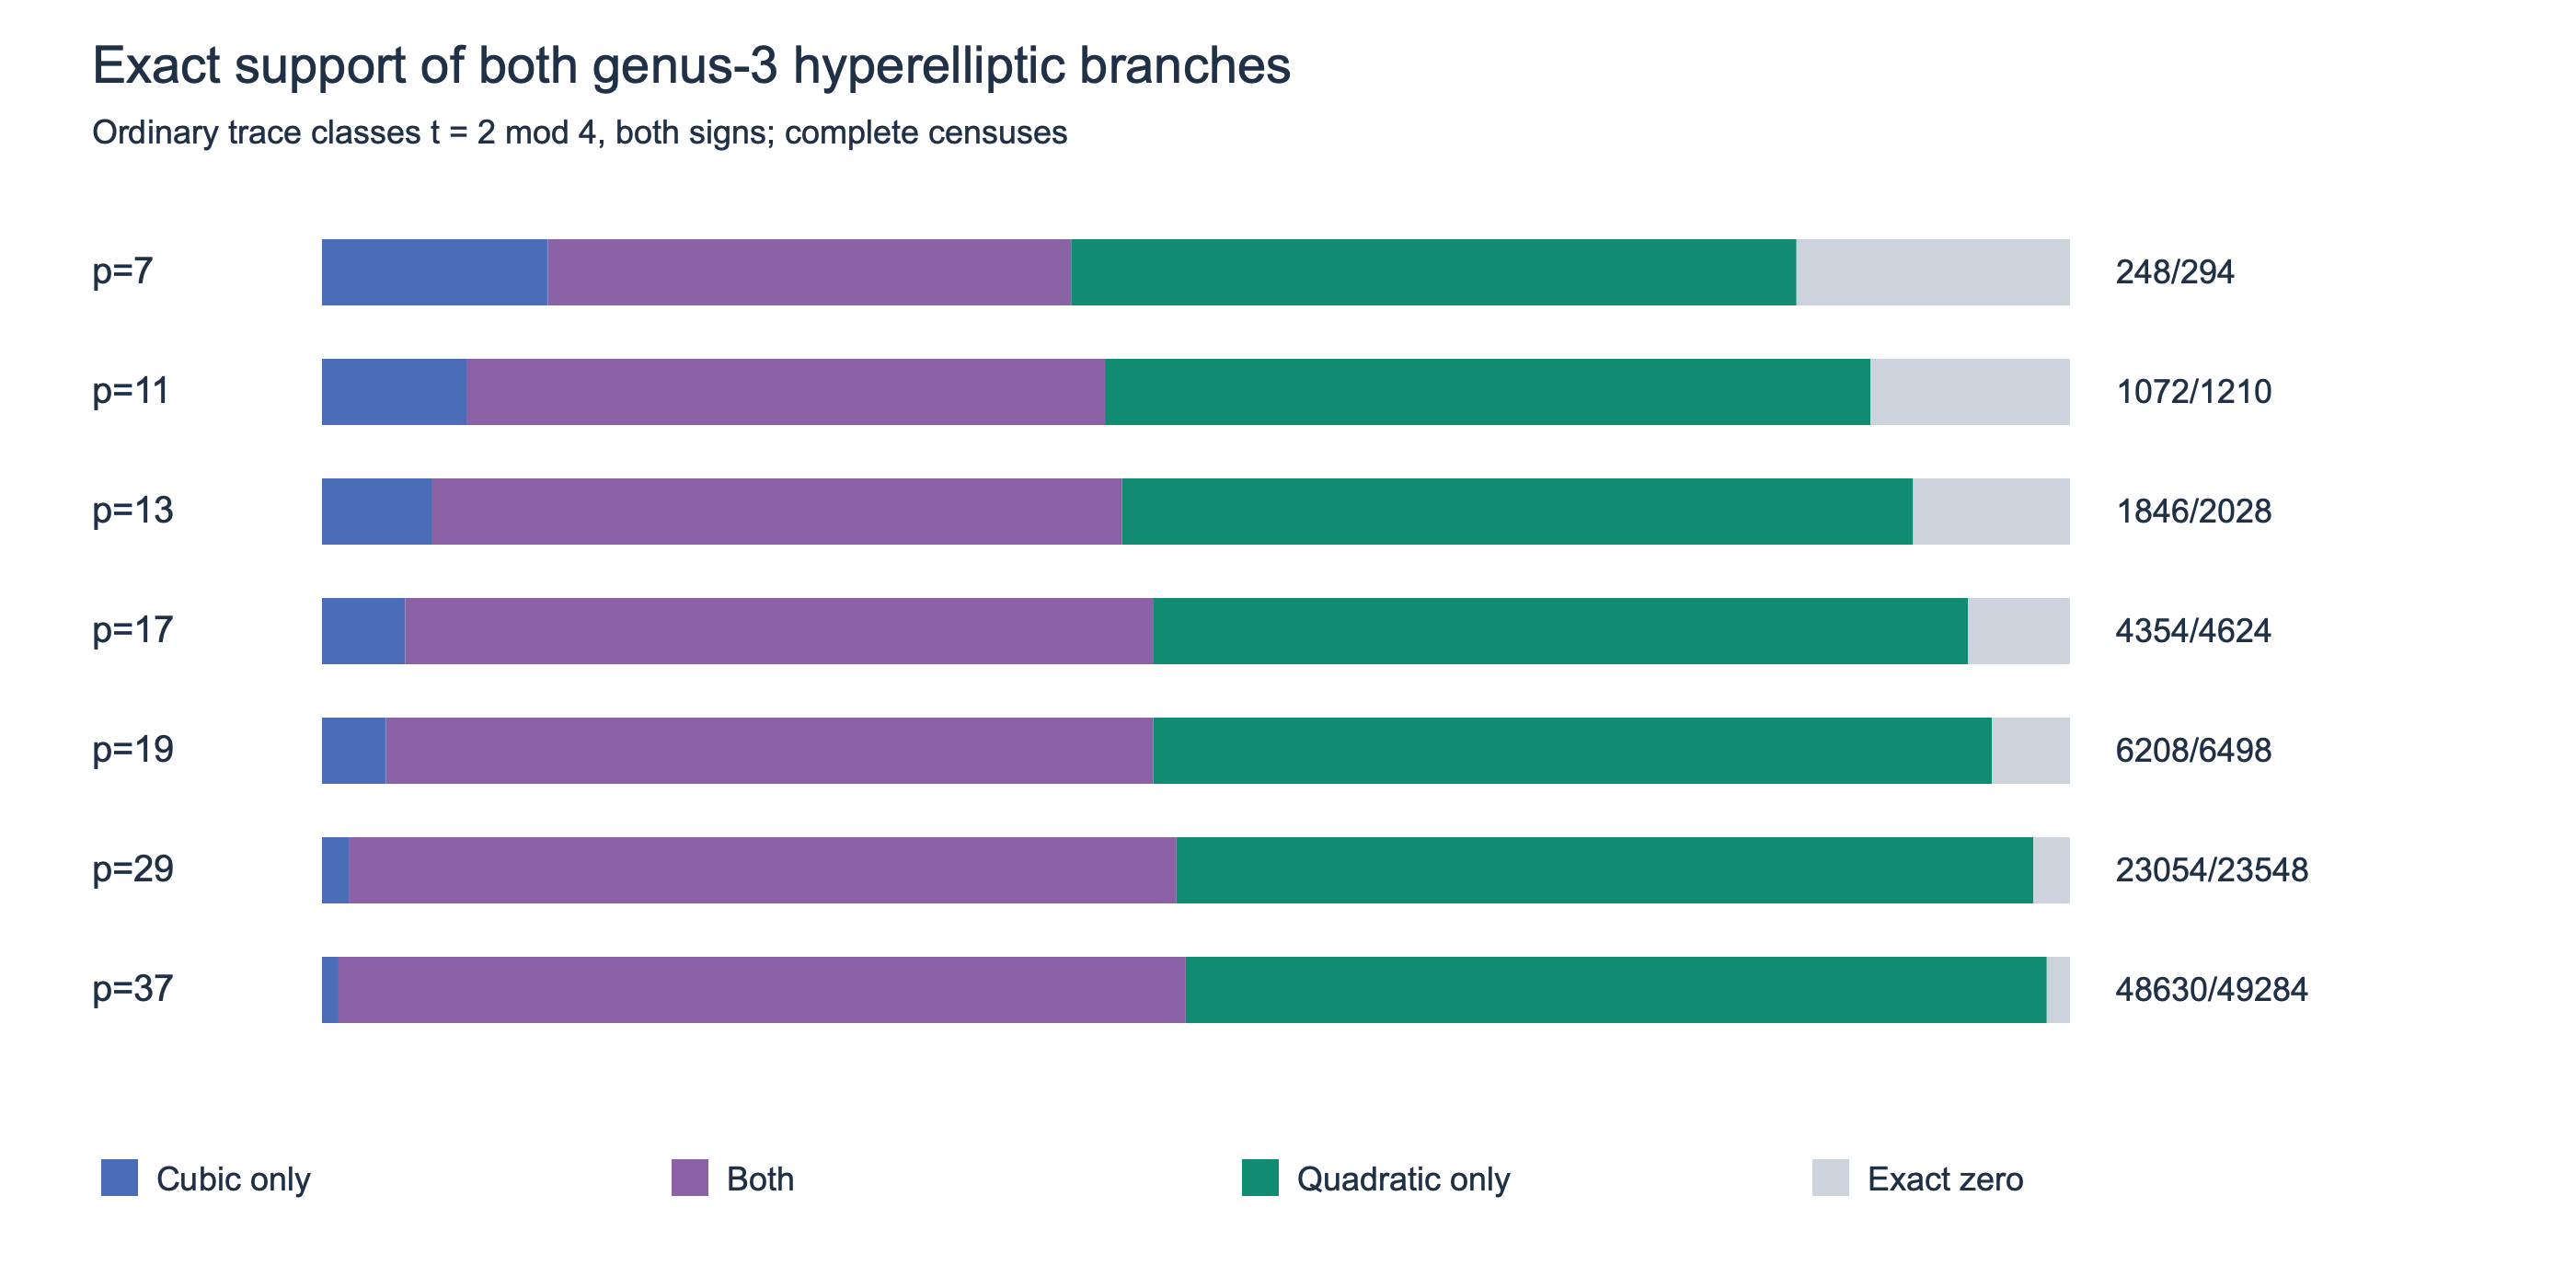
\includegraphics[width=0.95\linewidth]{coverage.png}
\caption{Complete ordinary trace-class support, partitioned by the two
branches. Each bar is a census, without sampling uncertainty.}\end{figure}
\begin{figure}[ht]\centering
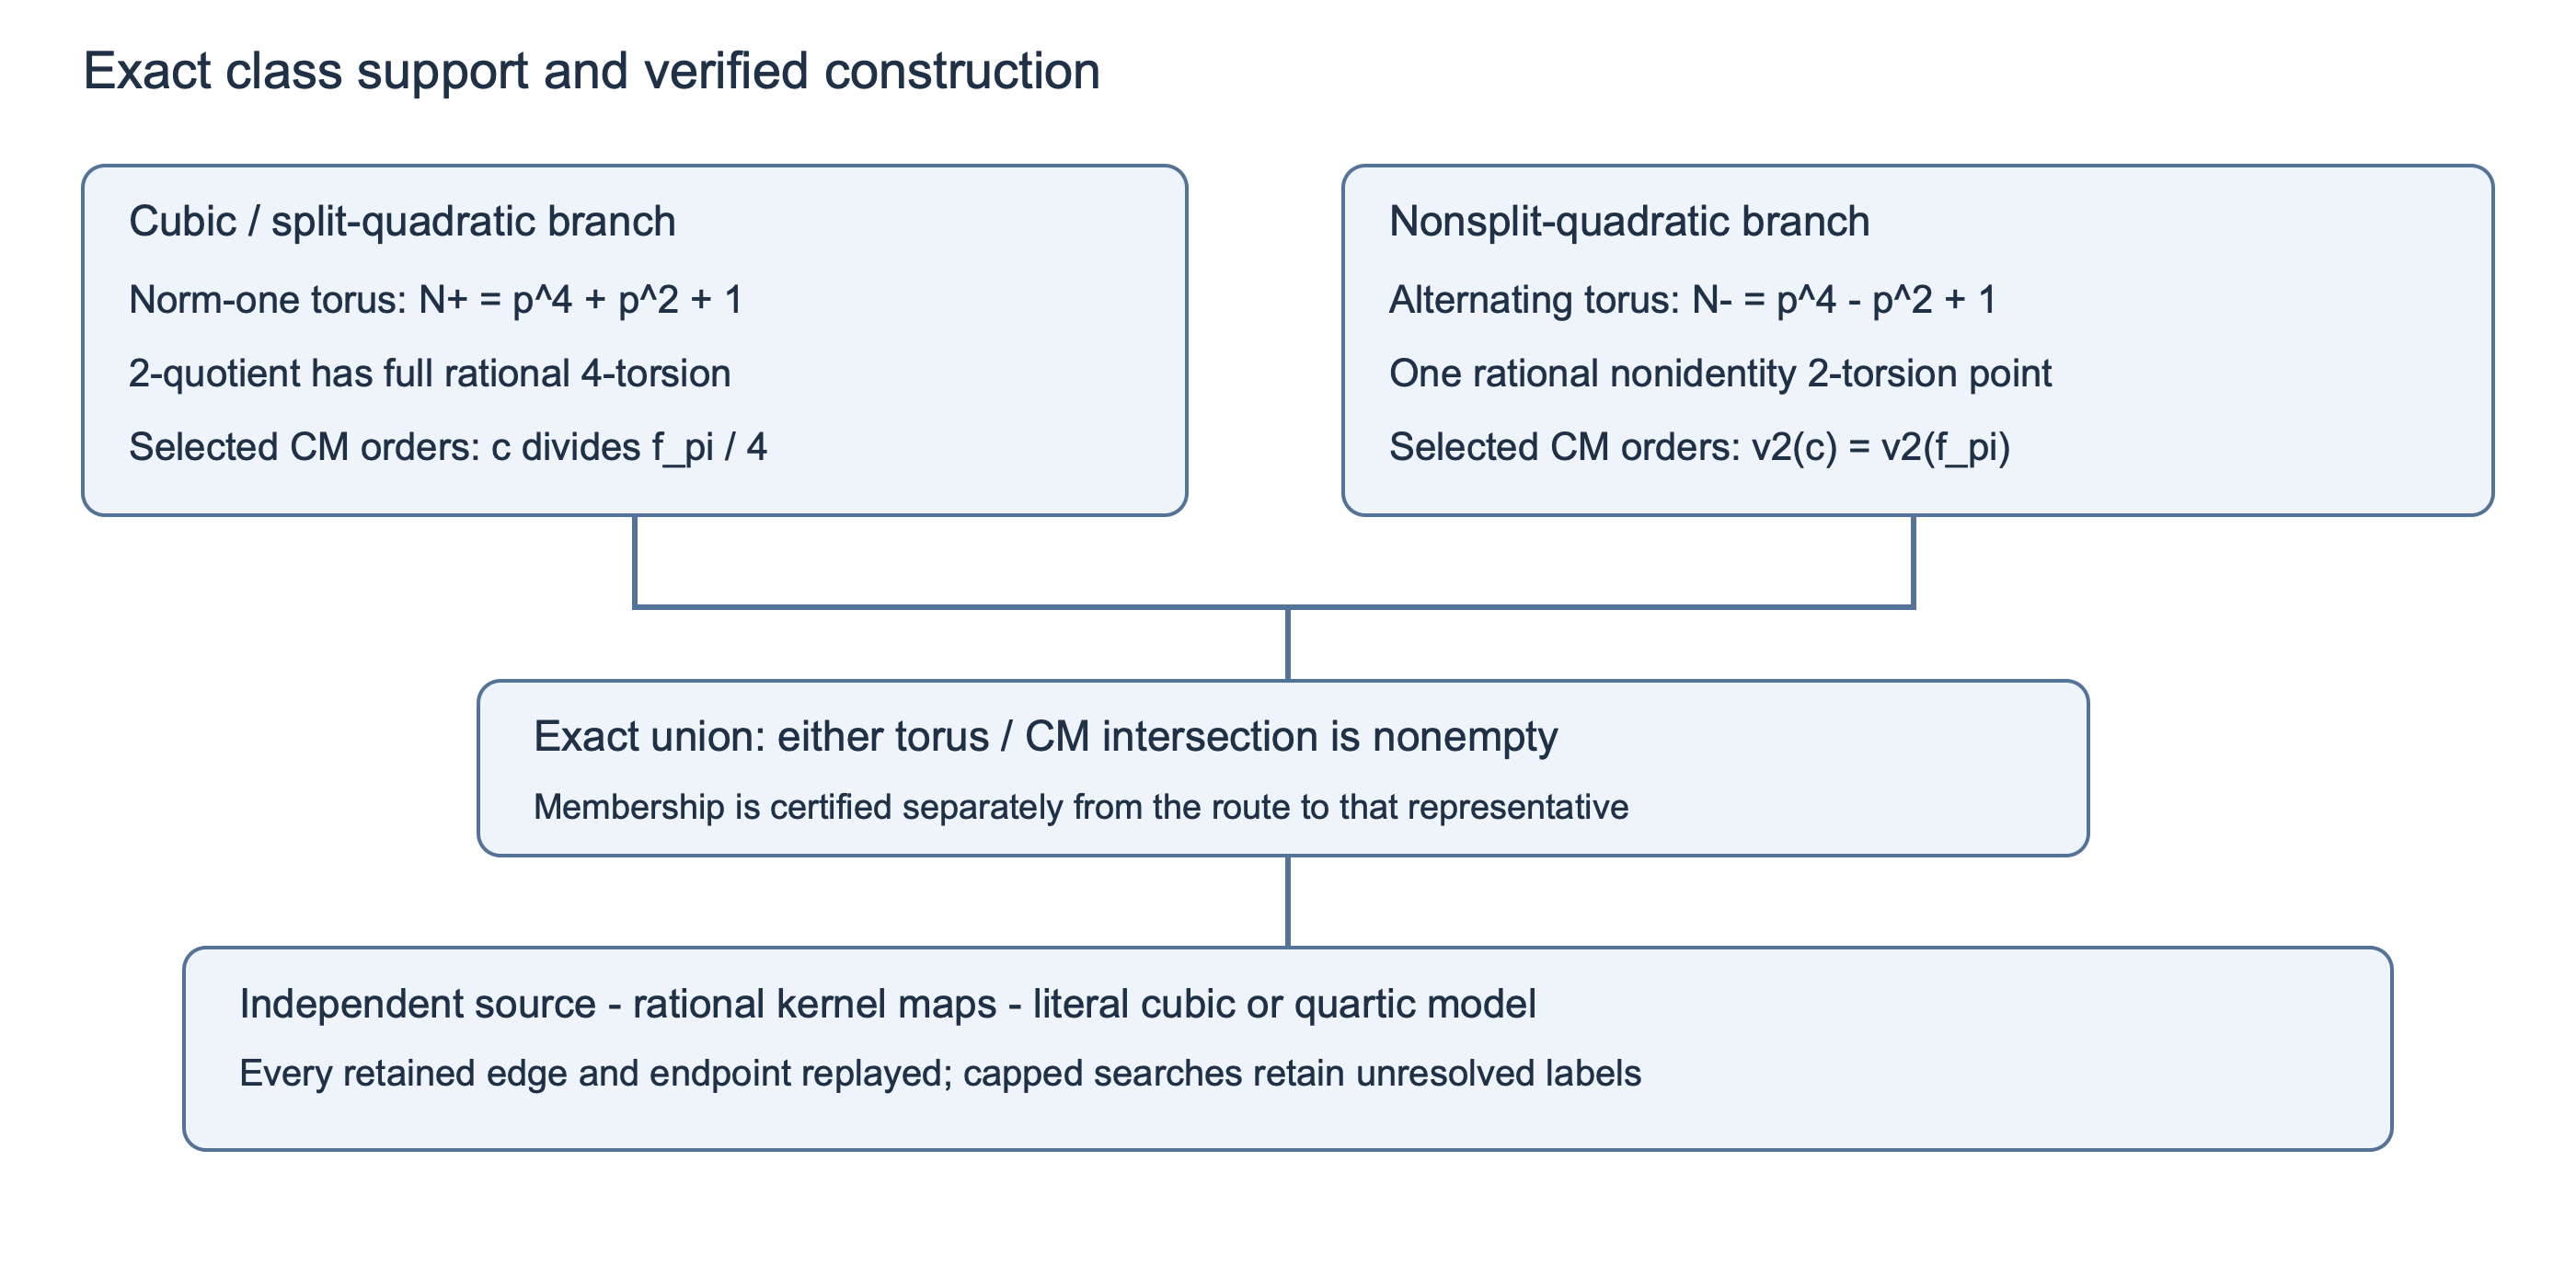
\includegraphics[width=0.95\linewidth]{two_branch_flow.png}
\caption{Exact support and constructive recognition use different data:
class intersections establish membership, and verified maps establish a route
from a specified independent source.}\end{figure}
\begin{figure}[ht]\centering
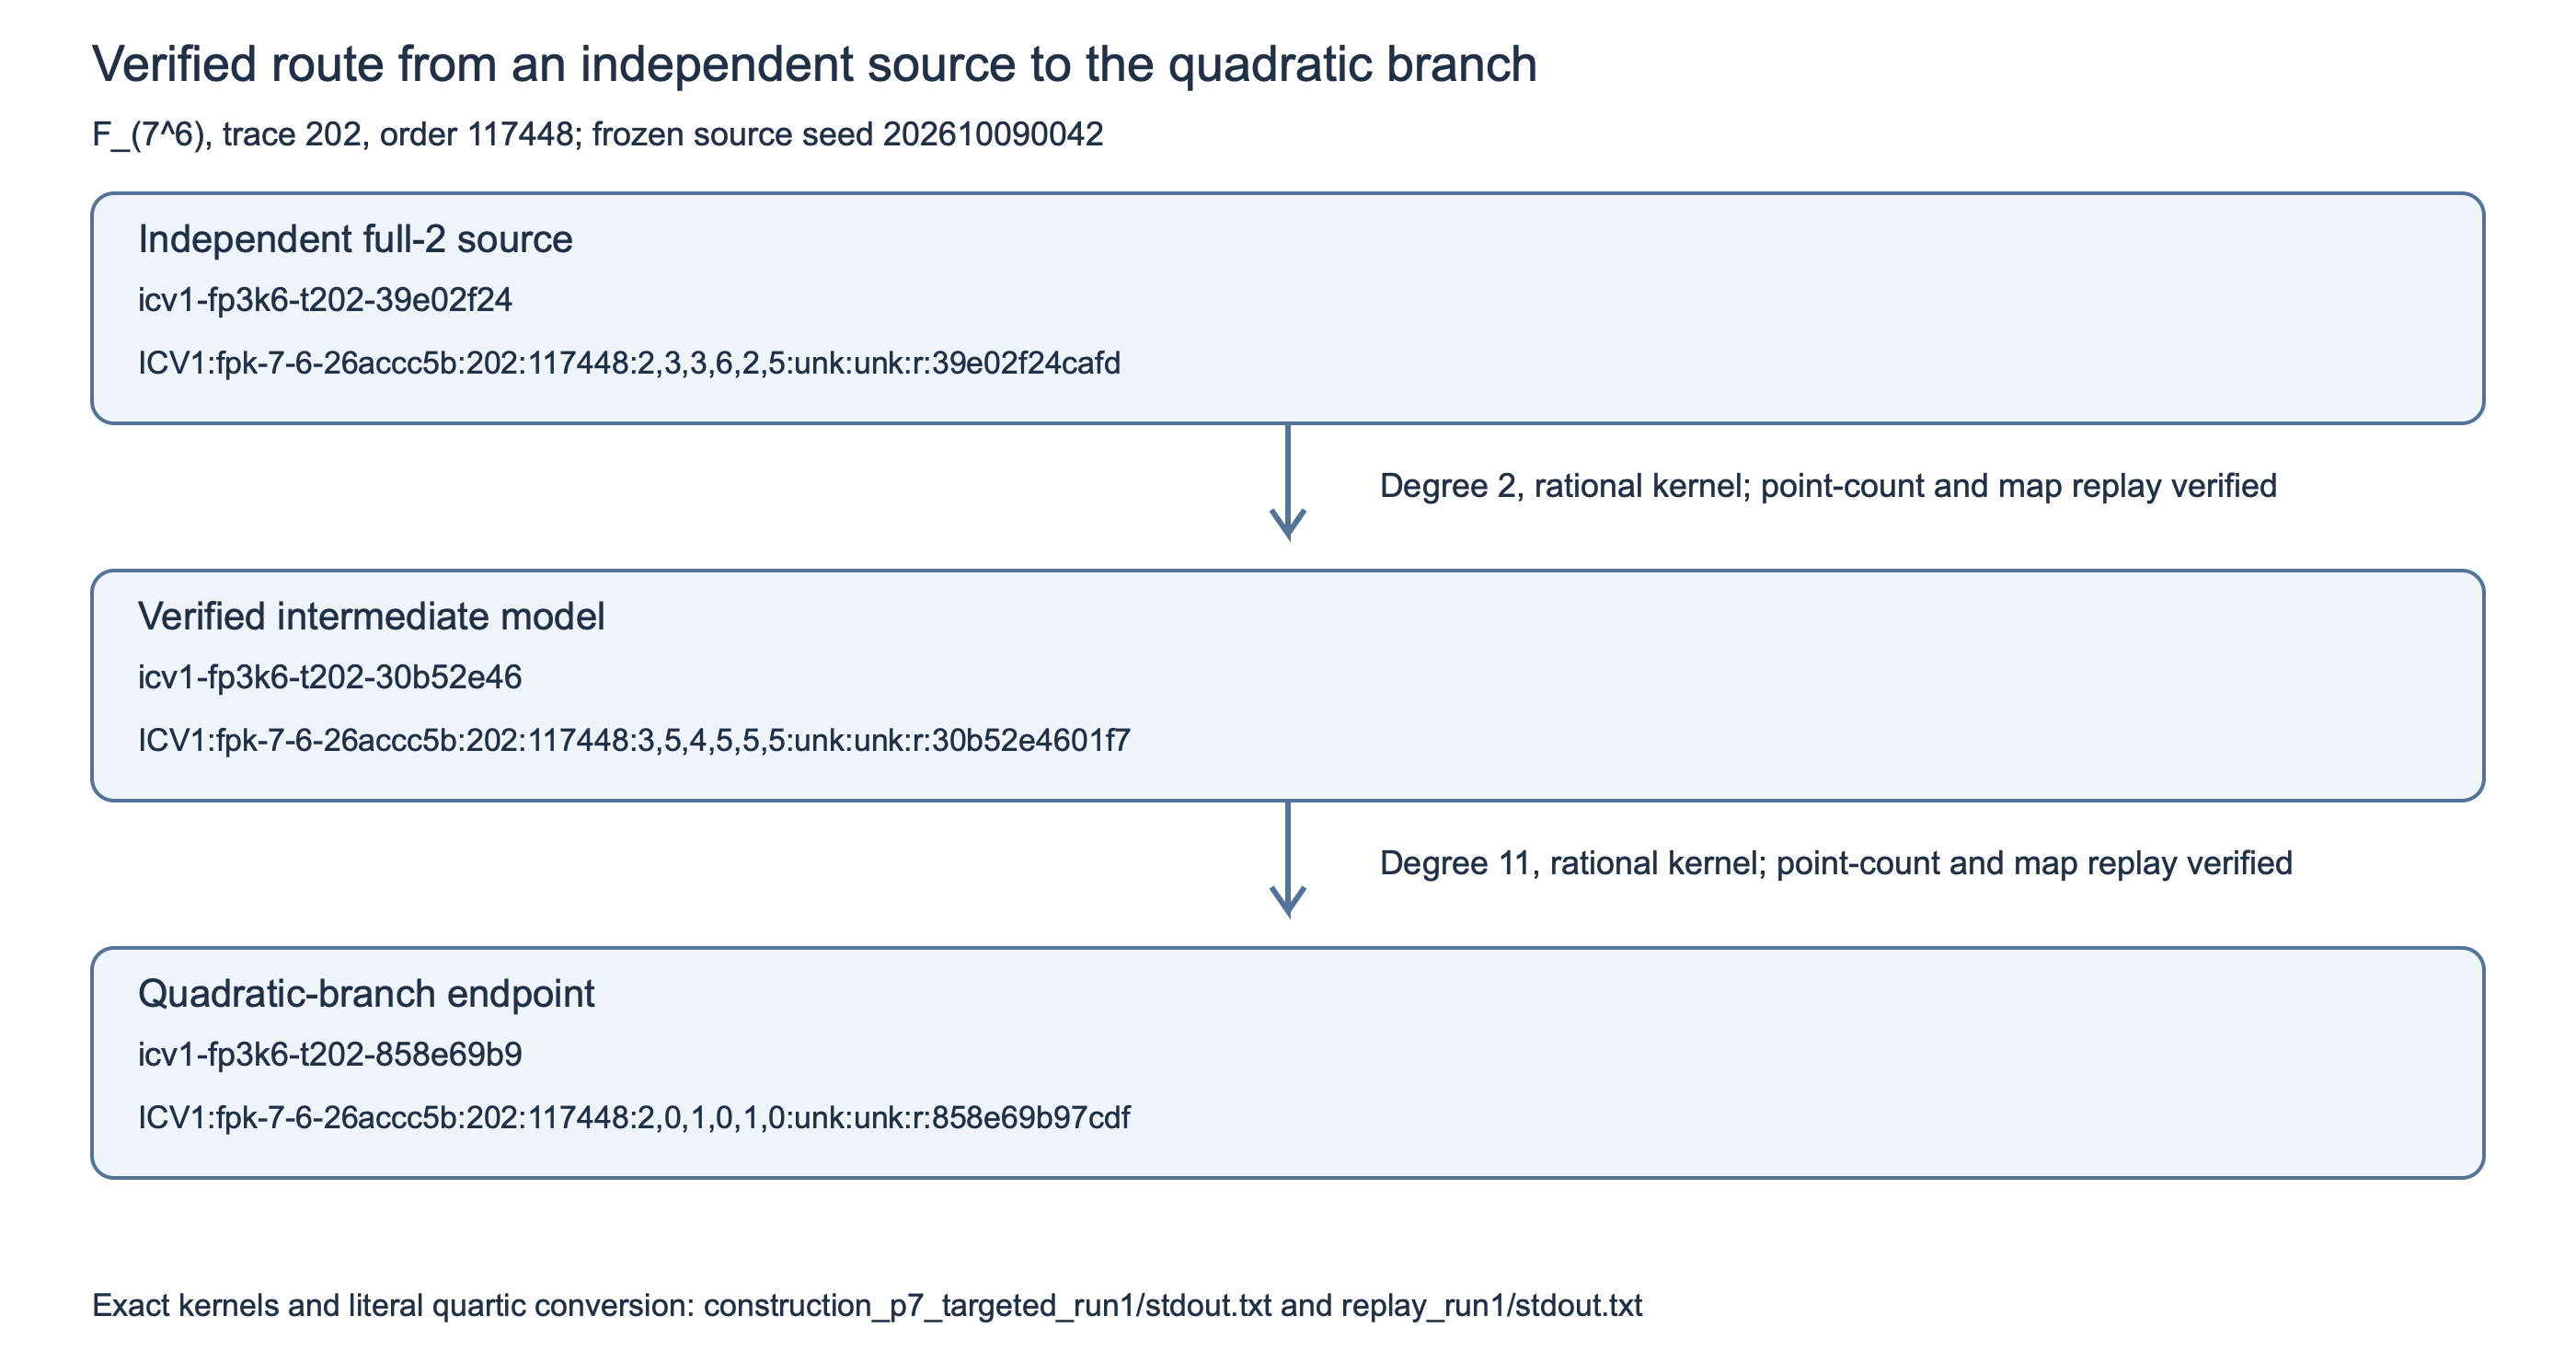
\includegraphics[width=0.95\linewidth]{verified_route.png}
\caption{A frozen independent source reaches a literal quadratic representative
through verified degree-2 and degree-11 maps. Full model identities and kernel
polynomials are retained in the independent replay.}\end{figure}

\section{192--252-bit fields and cost accounting}
The expanded search uses all 384 frozen degree-6 sources, 64 per field at
integer field bit lengths 192, 204, 216, 228, 240 and 252. Source moduli,
roots, counts and seeds are reused exactly; the two-branch search tests every
source, including those excluded by the cubic condition. It retains vertices
with either one or three rational nonidentity 2-torsion points and tests the
quadratic endpoint criterion on the former. The resource envelope is four GP
workers, 256 distinct invariants and 90 seconds per source, with a 240-second
parent cap and a 256 MiB initial stack. Every source keeps a separate raw
output, stderr, hash freeze and process receipt.

\begin{center}\begin{tabular}{rrrrrrr}\toprule
Bits & Degree & p & Sources & Closures & Caps & Visited\\\midrule
192 & 6 & 4294967291 & 64 & 48 & 16 & 6152\\
204 & 6 & 17179869143 & 64 & 44 & 20 & 6470\\
216 & 6 & 68719476731 & 64 & 43 & 21 & 6904\\
228 & 6 & 274877906899 & 64 & 48 & 16 & 5604\\
240 & 6 & 1099511627689 & 64 & 52 & 12 & 4692\\
252 & 6 & 4398046511093 & 64 & 45 & 19 & 6578\\
192 & 10 & 602233 & 32 & 28 & 4 & 2020\\
252 & 10 & 38543917 & 32 & 25 & 7 & 2964\\
192 & 14 & 13421 & 32 & 26 & 6 & 2138\\
252 & 14 & 262139 & 32 & 24 & 8 & 2834\\
\bottomrule\end{tabular}
\end{center}
All timings include the named phase's failed attempts. Setup, source checking,
search and final verification stay separate; they are resource measurements
on the shared Apple M4 Pro host, not isolated timing ratios. Direct membership
testing is a constant-degree root calculation and torus exponentiation.
Exact isogeny-class membership still requires the CM sets or an equivalent
complete oracle. The earlier 192-bit CM preflight retained the native
integer-conversion overflow on a 188-bit fundamental discriminant.
The complete torus method needs about $p^4/6$ retained models: roughly
$2^{125.4}$ at the 192-bit endpoint and $2^{165.4}$ at 252 bits.
These are parameter-count calculations, not measured construction times.

The existing degree-10 and degree-14 results remain separate higher-extension
evidence. The next theorem supplies their nonsplit reconstruction; the
genus-3 class theorem above retains domain $K/\F_{p^2}$ of degree three.
An additional 128 frozen independent degree-10/14 sources receives the same
two-branch bounded search. Sixteen separately constructed quartic controls
pass reconstruction, fresh point counts and independent recorded-coordinate
replay. Eight controls have $\gcd(q+1,N_-)=5$, so the simple inverse exponent
cannot supply their section. Their compositum covers have genera 25 and 161,
as specified below. The two population panels together retain all 512 sources.

\section{Constructive quadratic reconstruction in larger odd degrees}
\begin{theorem}[Quadratic-base Hilbert-90 reconstruction]
Let $q$ be odd, $n\ge3$ odd, $Q=q^n$, $K=\F_Q$, $L=\F_{Q^2}$,
$N_-=(Q+1)/(q+1)$ and $\lambda\in\mu_{N_-}(L)\setminus\{1\}$.
Choose a base-field nonsquare $d$ and $\beta^2=d$.
Put $\rho=\lambda^{q-1}$ and construct a nonzero $\gamma_0$ satisfying
$\gamma_0^{q^2}=\rho\gamma_0$. Then
\[
 r=\gamma_0^{q+1}/\lambda\in\F_q^\times,\qquad
 c\in\F_{q^2}^\times,\quad c^{q+1}=r^{-1},\qquad
 \gamma=c\gamma_0,\quad \alpha=\beta\frac{\gamma+1}{\gamma-1}
\]
construct $\alpha\in K\setminus\F_q$ with quartic invariant $j(\lambda)$.
This works even when $\gcd(q+1,N_-)>1$.
\end{theorem}
\begin{proof}
The norm of $\rho$ from $L$ to $\F_{q^2}$ is
$\lambda^{(Q^2-1)/(q+1)}=\lambda^{(Q-1)N_-}=1$.
Hilbert 90 supplies $\gamma_0$; the implementation uses the explicit
twisted trace on a complete prime-field basis and checks its Frobenius equation.
The equation also gives $r^q=r$. Iterating
$\gamma_0^q=r\lambda/\gamma_0$ through the odd cycle gives
$\gamma_0^{Q+1}=r\lambda^{N_-}=r$.
The quadratic-base-field norm is surjective. Writing $c=a+b\beta$, solve
$a^2-db^2=r^{-1}$ over $\F_q$. It follows that
$\gamma^{q+1}=\lambda$ and $\gamma^{Q+1}=1$.
The Cayley map therefore puts $\alpha$ in $K$, and $\alpha\in\F_q$ would
force $\lambda=1$. The four-root cross-ratio proves the invariant formula.
\end{proof}
The cleared norm identity has certificate \texttt{IDC1hdf7945dfb8d04948}.

For prime $n$, $\alpha\notin\F_q$ has a full orbit of length $n$.
The compositum of the $n$ conjugate quadratic function fields has degree
$2^n$ over $K(x)$: a square relation would give identical exponents at
consecutive orbit roots, hence all exponents equal, and the fixed base-field
branch pair forces that exponent to vanish because $n$ is odd.
There are $n+2$ branch points, each of index two. Riemann--Hurwitz gives
\[
 2g-2=-2\cdot2^n+(n+2)2^{n-1},\qquad
 g=1+2^{n-2}(n-2).
\]
The Frobenius action rotates the conjugate square roots, giving a descent
datum to $\F_q$. Thus this specified cover has genus 3, 25 or 161 at
$n=3,5,7$ respectively. This identifies the cover used by the extended
functional family; an alternative cover requires its own construction and cost.
The cleared Riemann--Hurwitz expression has certificate
\texttt{IDC1h545ec3e83899c369}.

\section{Separate larger-prime cubic continuation}
The finite cubic-census worker completed $p=61$ and $p=67$ with its
probabilistic two-point Hasse-BSGS counter and 5,000 independent PARI controls
per prime. Their retained status is diagnostic with GP control; they are
separate from the complete combined-family censuses above.
\begin{center}\begin{tabular}{rrrrr}\toprule
$p$ & Ordinary rows & Cubic positives & Depth-1 positives & High-depth zeros\\\midrule
61 & 223260 & 111084 & 0 & 546\\
67 & 296274 & 147496 & 0 & 640\\\bottomrule
\end{tabular}\end{center}
Every GP control lands in the corresponding positive set. The compressed
CSV replay hashes and all receipts are archived. The worker stopped before
$p=71$ at its storage preflight: 756,305,920 bytes were available against
1,173,957,184 required. After storage became available, a fresh finite queue
resumed at $p=71$, with 38,786,592,768 bytes available at launch. It retains
the same frozen binary, four CPU threads, the original per-prime storage
guard and the authorized range through $p=199$. The restart receipt records
the running service separately from the preserved stopped queue.

\begin{thebibliography}{9}
\bibitem{JV} A. Joux and V. Vitse. Cover and decomposition index calculus on
elliptic curves made practical. EUROCRYPT 2012, pp. 9--26.
\url{https://eprint.iacr.org/2011/020}.
\bibitem{MC} F. Momose and J. Chao. Elliptic curves with weak coverings over
cubic extensions of finite fields with odd characteristic, 2009.
\url{https://eprint.iacr.org/2009/236}.
\bibitem{Suth} A. V. Sutherland. Isogeny volcanoes. MIT 18.783,
Lecture 22, Fall 2023.
\url{https://math.mit.edu/classes/18.783/2023/LectureNotes22.pdf}.
\end{thebibliography}
\end{document}
